% Created 2016-08-16 Tue 05:14
\documentclass[11pt]{article}
\usepackage[utf8]{inputenc}
\usepackage[T1]{fontenc}
\usepackage{fixltx2e}
\usepackage{graphicx}
\usepackage{longtable}
\usepackage{float}
\usepackage{wrapfig}
\usepackage{rotating}
\usepackage[normalem]{ulem}
\usepackage{amsmath}
\usepackage{textcomp}
\usepackage{marvosym}
\usepackage{wasysym}
\usepackage{amssymb}
\usepackage{hyperref}
\tolerance=1000
\author{XU Sheng}
\date{8 Aug 2016}
\title{Data Analysis}
\hypersetup{
  pdfkeywords={},
  pdfsubject={},
  pdfcreator={Emacs 24.5.1 (Org mode 8.2.10)}}
\begin{document}

\maketitle
\tableofcontents


\section{Re-assign values to the demographically information}
\label{sec-1}
\subsection{Age}
\label{sec-1-1}
Age = 1, for age <= 35; Age = 2, otherwise
\subsection{Education}
\label{sec-1-2}
Education = 1 for Education <= 2; Education = 2, otherwise

\section{Grouping}
\label{sec-2}
\begin{center}
\begin{tabular}{llrrrrr}
Group name & location & Age & Edu & Sex & Marriage & Size\\
\hline
A.1.1.1.1 & A & 1 & 1 & 1 & 1 & 192\\
A.1.1.1.2 & A & 1 & 1 & 1 & 2 & 207\\
A.1.1.2.1 & A & 1 & 1 & 2 & 1 & 115\\
A.1.1.2.2 & A & 1 & 1 & 2 & 2 & 314\\
A.1.2.1.1 & A & 1 & 2 & 1 & 1 & 373\\
A.1.2.1.2 & A & 1 & 2 & 1 & 2 & 365\\
A.1.2.2.1 & A & 1 & 2 & 2 & 1 & 227\\
A.1.2.2.2 & A & 1 & 2 & 2 & 2 & 378\\
A.2.1.1.1 & A & 2 & 1 & 1 & 1 & 22\\
A.2.1.1.2 & A & 2 & 1 & 1 & 2 & 3\\
A.2.1.2.1 & A & 2 & 1 & 2 & 1 & 147\\
A.2.1.2.2 & A & 2 & 1 & 2 & 2 & 7\\
A.2.2.1.1 & A & 2 & 2 & 1 & 1 & 283\\
A.2.2.1.2 & A & 2 & 2 & 1 & 2 & 3\\
A.2.2.2.1 & A & 2 & 2 & 2 & 1 & 266\\
A.2.2.2.2 & A & 2 & 2 & 2 & 2 & 13\\
B.1.1.1.1 & B & 1 & 1 & 1 & 1 & 127\\
B.1.1.1.2 & B & 1 & 1 & 1 & 2 & 34\\
B.1.1.2.1 & B & 1 & 1 & 2 & 1 & 73\\
B.1.1.2.2 & B & 1 & 1 & 2 & 2 & 111\\
B.1.2.1.1 & B & 1 & 2 & 1 & 1 & 75\\
B.1.2.1.2 & B & 1 & 2 & 1 & 2 & 151\\
B.1.2.2.1 & B & 1 & 2 & 2 & 1 & 56\\
B.1.2.2.2 & B & 1 & 2 & 2 & 2 & 159\\
B.2.1.1.1 & B & 2 & 1 & 1 & 1 & 183\\
B.2.1.1.2 & B & 2 & 1 & 1 & 2 & 5\\
B.2.1.1.1 & B & 2 & 1 & 2 & 1 & 104\\
B.2.1.1.2 & B & 2 & 1 & 2 & 2 & 4\\
B.2.2.2.1 & B & 2 & 2 & 1 & 1 & 54\\
B.2.2.2.2 & B & 2 & 2 & 1 & 2 & 3\\
B.2.2.1.1 & B & 2 & 2 & 2 & 1 & 58\\
B.2.2.1.2 & B & 2 & 2 & 2 & 2 & 2\\
C.1.1.2.1 & C & 1 & 1 & 1 & 1 & 114\\
C.1.1.2.2 & C & 1 & 1 & 1 & 2 & 95\\
C.1.1.1.1 & C & 1 & 1 & 2 & 1 & 56\\
C.1.1.1.2 & C & 1 & 1 & 2 & 2 & 115\\
C.1.2.2.1 & C & 1 & 2 & 1 & 1 & 177\\
C.1.2.2.2 & C & 1 & 2 & 1 & 2 & 460\\
C.1.2.1.1 & C & 1 & 2 & 2 & 1 & 73\\
C.1.2.1.2 & C & 1 & 2 & 2 & 2 & 187\\
C.2.1.2.1 & C & 2 & 1 & 1 & 1 & 507\\
C.2.1.2.2 & C & 2 & 1 & 1 & 2 & 4\\
C.2.1.1.1 & C & 2 & 1 & 2 & 1 & 228\\
C.2.1.1.2 & C & 2 & 1 & 2 & 2 & 7\\
C.2.2.2.1 & C & 2 & 2 & 1 & 1 & 81\\
C.2.2.2.2 & C & 2 & 2 & 1 & 2 & 1\\
C.2.2.1.1 & C & 2 & 2 & 2 & 1 & 81\\
C.2.2.1.2 & C & 2 & 2 & 2 & 2 & 3\\
\end{tabular}
\end{center}

\section{Total score comparisons}
\label{sec-3}

\begin{center}
\begin{tabular}{rlll}
p-value & A vs B & A vs C & B vs C\\
Groups: &  &  & \\
\hline
1.1.1.1 & 0.01 & 0.00 & \textbf{0.45}\\
1.1.1.2 & \textbf{0.18} & \textbf{0.39} & \textbf{0.07}\\
1.1.2.1 & \textbf{0.15} & \textbf{0.72} & \textbf{0.12}\\
1.1.2.2 & \textbf{0.55} & \textbf{0.22} & \textbf{0.61}\\
1.2.1.1 & \textbf{0.58} & 0.00 & 0.00\\
1.2.1.2 & \textbf{0.20} & 0.00 & 0.00\\
1.2.2.1 & \textbf{0.09} & \textbf{0.21} & \textbf{0.81}\\
1.2.2.2 & \textbf{0.51} & 0.00 & 0.00\\
2.1.1.1 & \textbf{0.92} & \textbf{0.94} & \textbf{0.97}\\
2.1.1.2 & \textbf{0.72} & \textbf{0.67} & \textbf{0.88}\\
2.1.2.1 & \textbf{0.08} & \textbf{0.44} & 0.01\\
2.1.2.2 & \textbf{0.58} & \textbf{0.64} & \textbf{0.93}\\
2.2.1.1 & 0.00 & \textbf{0.13} & \textbf{0.12}\\
2.2.1.2 & \textbf{0.68} & - & -\\
2.2.2.1 & \textbf{0.27} & \textbf{0.39} & \textbf{0.48}\\
2.2.2.2 & 0.01 & 0.00 & 0.00\\
\end{tabular}
\end{center}

The bold p-value numbers show that the total scores of the majority groups have no significant difference among location A, B, and C.

\section{Analysis after combining ABC together}
\label{sec-4}
Combine the group A, B, and C into one group names group P. The following results are based on the comparison between group P and AH.
Sub group naming rule: The Capital letter(s) means the group name, the number mean the total score level. For example, the sub-group AH1 means the observations in it think themselves have no psychological illness and the total score level is 1.

\subsection{Demographic factors difference}
\label{sec-4-1}
\begin{center}
\begin{tabular}{rllllll}
Sub-groups: & P0, N=2311 & P1, N=1737 & P2, N=2582 & AH0, N=11036 & AH1, N=2852 & AH2, N=1690\\
Demographics & Mean ± SD or N (\%) &  &  &  &  & \\
\hline
Sex &  &  &  &  &  & \\
1 & 1372 (36.05) & 943 (24.78) & 1491 (39.17) & 4418 (73.41) & 1010 (16.78) & 590 (9.8)\\
2 & 939 (33.25) & 794 (28.12) & 1091 (38.63) & 6618 (69.23) & 1842 (19.27) & 1100 (11.51)\\
Age (years) & 33.78 +- 12.52 & 35.24 +- 13 & 31.12 +- 11.42 & 34.33 +- 8.51 & 33.5 +- 8.19 & 33.46 +- 8.17\\
Age level &  &  &  &  &  & \\
1 & 1440 (33.4) & 1005 (23.31) & 1866 (43.28) & 6104 (69.02) & 1711 (19.35) & 1029 (11.64)\\
2 & 871 (37.56) & 732 (31.57) & 716 (30.88) & 4932 (73.24) & 1141 (16.94) & 661 (9.82)\\
Edu level &  &  &  &  &  & \\
1 & 944 (30.89) & 834 (27.29) & 1278 (41.82) & 5731 (71.47) & 1478 (18.43) & 810 (10.1)\\
2 & 1367 (38.25) & 903 (25.27) & 1304 (36.49) & 5305 (70.18) & 1374 (18.18) & 880 (11.64)\\
Marriage &  &  &  &  &  & \\
1 & 1369 (35.06) & 1145 (29.32) & 1391 (35.62) & 7783 (71.87) & 1913 (17.66) & 1134 (10.47)\\
2 & 916 (34.82) & 563 (21.4) & 1152 (43.79) & 3070 (69.07) & 867 (19.51) & 508 (11.43)\\
3 & 4 (40) & 3 (30) & 3 (30) & 0 (NaN) & 0 (NaN) & 0 (NaN)\\
4 & 22 (26.19) & 26 (30.95) & 36 (42.86) & 183 (60.4) & 72 (23.76) & 48 (15.84)\\
\end{tabular}
\end{center}
\subsection{Psychological factors difference}
\label{sec-4-2}


\begin{center}
\begin{tabular}{lllllll}
Sub-groups: & P0, N=2311 & P1, N=1737 & P2, N=2582 & AH0, N=11036 & AH1, N=2852 & AH2, N=1690\\
Psychological factors & Mean ± SD or N (\%) &  &  &  &  & \\
\hline
So & 1.38 +- 0.39 & 1.82 +- 0.5 & 2.48 +- 0.74 & 1.39 +- 0.35 & 2.09 +- 0.45 & 2.98 +- 0.77\\
Ocd & 1.62 +- 0.39 & 2.3 +- 0.47 & 3.17 +- 0.62 & 1.54 +- 0.36 & 2.29 +- 0.35 & 3.12 +- 0.6\\
IS & 1.39 +- 0.34 & 2.03 +- 0.49 & 2.99 +- 0.7 & 1.3 +- 0.29 & 1.98 +- 0.34 & 2.85 +- 0.64\\
Dep & 1.49 +- 0.37 & 2.3 +- 0.43 & 3.32 +- 0.62 & 1.35 +- 0.31 & 2.14 +- 0.32 & 3.07 +- 0.62\\
Anx & 1.51 +- 0.4 & 2.25 +- 0.48 & 3.19 +- 0.66 & 1.34 +- 0.27 & 2.05 +- 0.3 & 3 +- 0.65\\
Ho & 1.42 +- 0.42 & 1.97 +- 0.59 & 2.79 +- 0.88 & 1.27 +- 0.29 & 1.9 +- 0.44 & 2.86 +- 0.83\\
PA & 1.24 +- 0.33 & 1.65 +- 0.54 & 2.44 +- 0.8 & 1.15 +- 0.21 & 1.61 +- 0.38 & 2.43 +- 0.81\\
PI & 1.29 +- 0.33 & 1.79 +- 0.47 & 2.7 +- 0.76 & 1.23 +- 0.28 & 1.82 +- 0.39 & 2.7 +- 0.74\\
Psy & 1.3 +- 0.27 & 1.81 +- 0.36 & 2.69 +- 0.62 & 1.23 +- 0.22 & 1.8 +- 0.3 & 2.63 +- 0.67\\
Ai & 1.65 +- 0.54 & 2.23 +- 0.56 & 2.94 +- 0.68 & 1.35 +- 0.34 & 2.01 +- 0.44 & 2.83 +- 0.69\\
\end{tabular}
\end{center}

\subsection{Psychological factors correlations}
\label{sec-4-3}
\subsubsection{Sub-group P0}
\label{sec-4-3-1}
\begin{figure}[htb]
\centering
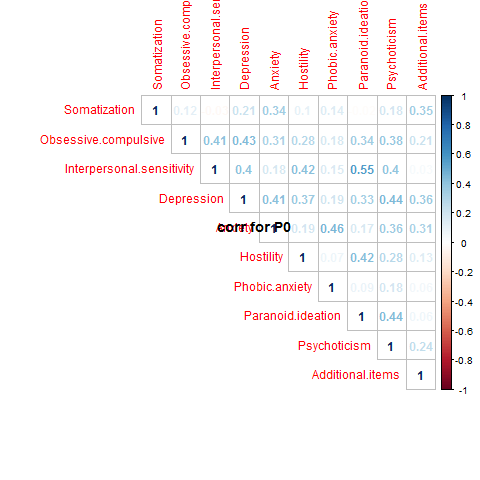
\includegraphics[width=.9\linewidth]{/home/tsui/Documents/psydata/corr1.png}
\label{P0-corrplot}
\end{figure} 

\subsubsection{Sub-group P1}
\label{sec-4-3-2}
\begin{figure}[htb]
\centering
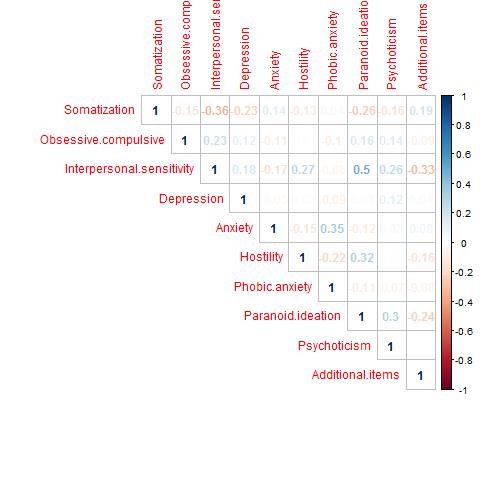
\includegraphics[width=.9\linewidth]{/home/tsui/Documents/psydata/corr2.png}
\label{P2-corrplot}
\end{figure}
\subsubsection{Sub-group P2}
\label{sec-4-3-3}
\begin{figure}[htb]
\centering
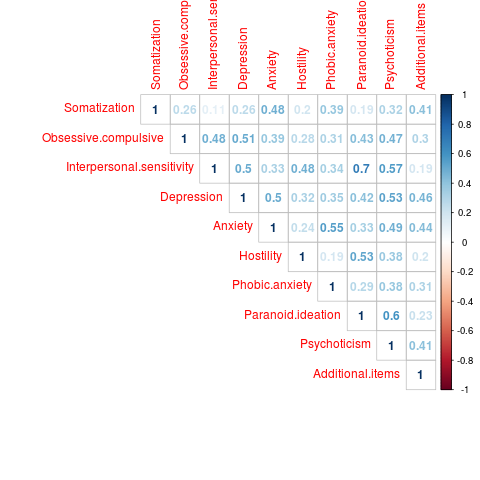
\includegraphics[width=.9\linewidth]{/home/tsui/Documents/psydata/corr3.png}
\label{P3-corrplot}
\end{figure}
\subsubsection{Sub-group AH0}
\label{sec-4-3-4}
\begin{figure}[htb]
\centering
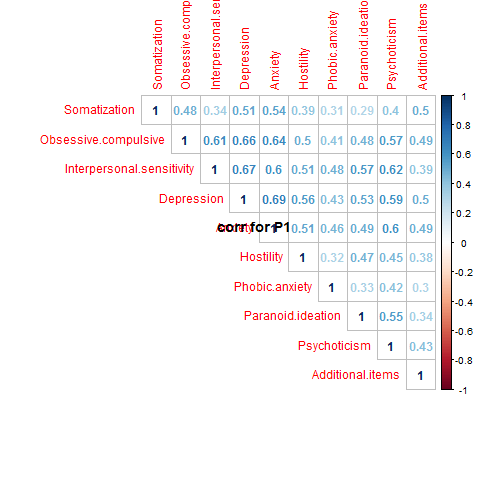
\includegraphics[width=.9\linewidth]{/home/tsui/Documents/psydata/corr4.png}
\label{AH0-corrplot}
\end{figure}
\subsubsection{Sub-group AH1}
\label{sec-4-3-5}
\begin{figure}[htb]
\centering
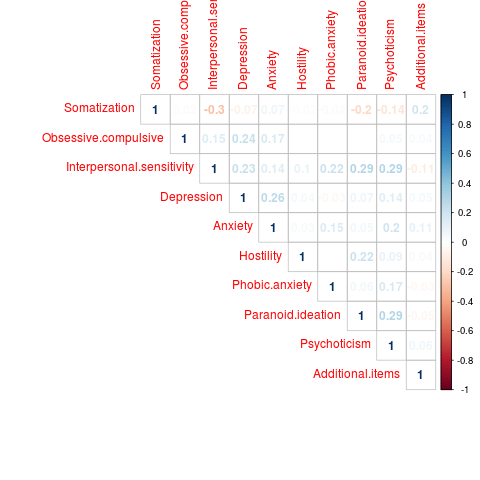
\includegraphics[width=.9\linewidth]{/home/tsui/Documents/psydata/corr5.png}
\label{AH1-corrplot}
\end{figure}
\subsubsection{Sub-group AH2}
\label{sec-4-3-6}
\begin{figure}[htb]
\centering
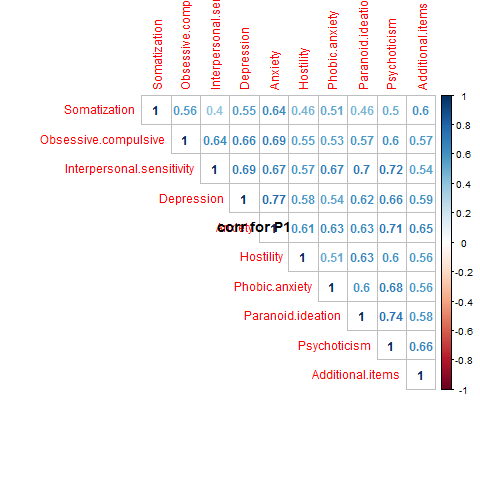
\includegraphics[width=.9\linewidth]{/home/tsui/Documents/psydata/corr6.png}
\label{AH2-corrplot}
\end{figure}
% Emacs 24.5.1 (Org mode 8.2.10)
\end{document}
